\chapter{Implementacja}
\label{cha:implementacja}

W niniejszym rozdziale zostanie bardziej szczegółowo opisana realizacja komponentów
gry opisanych w części \ref{cha:projekt}.

\section{Wyjaśnienie dotyczące zamieszczonych diagramów UML}
\label{sec:uml}

W niniejszej części pracy będzie wykorzystywany język UML do przedstawienia implementacji
poszczególnych komponentów. Język ten pomimo swej użyteczności nie jest jednak idealny
do przedstawiania kodu programu stworzonego w JavaScript, dlatego trzeba na początku
wyjaśnić kilka nieścisłości.

UML operuje na pojęciach znanych z języków obiektowych, wykorzystujących klasy. Są to pojęcia
takie jak klasa, interfejs, metoda, dziedziczenie itp. Jednakże w JavaScript obiektowość
jest realizowana przez prototypy\footnote{Więcej na ten temat paradygmatu programowania
  przez prototypowanie w \cite{js-definitive}.}, a więc
terminy te nie występują w samym języku. Język ten jednak jest na tyle elastyczny, że możliwa
jest realizacja konstrukcji odpowiadających im. Dodatkowo, często stosuje się znaczniki
JSDoc\footnote{JSDoc -- język używany do dokumentowania kodu w JavaScript podobny do
  Javadoc, znanego z Javy.}, aby jawnie wskazać takie konstrukcje.

W dalszej części opisu, pojęcia te będą stosowane zgodnie z terminologią UML.

\section{Użyte narzędzia}
\label{sec:uzyteNarzedzia}

\subsection{Google Closure}
\label{ssec:googleClosure}

\section{Wielowątkowość}
\label{sec:wielowatkowosc}

Realizacja wielowątkowości w Web Workers wymaga, aby poszczególne wątki komunikowały się
jedynie za pomocą wiadomości mogących zawierać jedynie niektóre typy danych (zakazane
jest na przykład przesyłanie obiektów HTML DOM). Współdzielenie
kodu oraz pamięci jest niemożliwe, nie można więc wywołać funkcji "pomiędzy" workerami.

Te ograniczenia sprawiają, że należy z góry zaplanować jak zostanie podzielony
kod pomiędzy wątki. Jest to jednak rozwiązanie mało elastyczne. Trudno przełączać
się pomiędzy wersją jedno i wielowątkową w celu porównania wydajności i łatwiejszego
wyszukiwania błędów.
Dodatkowo wysyłanie komunikatów jest mniej wygodne niż proste wywołanie funkcji.

W WebArena został więc zaimplementowana wysokopoziomowa biblioteka do obsługi Web Workers,
wykorzystująca elastyczność języka JavaScript.

Oto jej cechy:

\subsection{Zdalne wywoływanie metod}
\label{ssec:zdalneWywolanie}
Po zarejestrowaniu obiektu w jednym workerze, biblioteka umożliwia utworzenie obiektu
proxy w drugim workerze na podstawie podanego interfejsu \footnote{JavaScript jest językiem
  bezklasowym, więc nie ma tam pojęcia tradycyjnego interfejsu (jak np. w języku Java, czy C\#).
  W związku z tym przyjęło się deklarować interfejs po prostu jako obiekt z pustymi metodami.}.
Dzięki temu komunikacja
pomiędzy workerami jest ukryta pod postacią zwykłego wywołania metody. Dodatkowo
obsługiwane jest przekazywanie funkcji jako tzw. callback, co na poziomie Web Workers
jest niemożliwe. Jest to system podobny do zdalnego wywoływania metod (np. RMI w języku Java),
jednak prostszy w użyciu, dzięki dynamicznemu charakterowi języka JavaScript.

Zalety takiego systemu:
\begin{itemize}
\item prostota użycia -- wystarczy zadeklarować interfejs dla obiektu, z proxy zostanie
  utworzone automatycznie,
\item możliwość przekazywania funkcji jako argumentu,
\item łatwe przełączanie pomiędzy trybem jedno i wielowątkowym (wystarczy zamiast proxy podstawić
  prawdziwy obiekt.
\end{itemize}

\subsection{Zdarzenia}
Biblioteka może być użyta również do globalnej (międzywątkowej) obsługi zdarzeń. 

Często jeden z komponentów jest zainteresowany zdarzeniem zachodzącym w innym komponencie.
Jeśli jednak pracują one w innych workerach, przekazanie funkcji jako callback jest
niemożliwe. Dlatego trzeba użyć warstwy pośredniczącej. W przypadku WebArena warstwa ta
umożliwia zarejestrowanie funkcji mającej reagować na zdarzenia oraz powiadamianie o występujących
zdarzeniach pomiędzy wątkami.

\subsection{Pule wątków}
\label{ssec:puleWatkow}
Pula wątków (Thread pool) jest to grupa wątków do których można szybko oddelegować wykonanie
małej części logiki bez konieczności tworzenia nowego wątku.

Tworzenie wątku może potrwać na tyle długo, aby zniweczyć wszelkie korzyści wynikające z oddelegowania
części pracy na osobny rdzeń procesora. Dodatkowo API Web Workers z reguły wymusza, aby pliki
z kodem źródłowym były z góry
przydzielone do konkretnego wątku. Proste przekazanie funkcji do wykonania w innym workerze nie zadziała.

Dlatego kolejnym zadaniem wykonywanym przez omawianą bibliotekę jest obejście tego ograniczenia, w celu
umożliwienia oddelegowania wykonania danej funkcji do puli wątków. Dodatkowo zadania takie są automatycznie
kolejkowane, a po ich wykonaniu wyniki zwracane do wywołującego wątku.

\subsection{Implementacja biblioteki}

\begin{figure}[h]
  \centering
  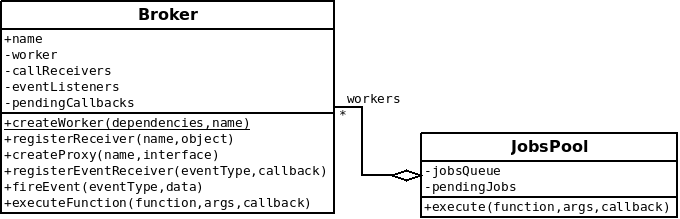
\includegraphics[scale=0.6]{zasoby/rozdzial31/broker}  
  \caption{Uproszczony diagram UML biblioteki}
  \label{fig:broker}
\end{figure}

Diagram \ref{fig:broker} przedstawia w uproszczeniu implementację omawianej biblioteki. Składa się ona
z dwóch głównych klas znajdujących się na diagramie oraz kilku mniej istotnych, które zostały pominięte
dla zachowania czytelności. Klasa Broker jest klasą najważniejszą i odpowiada za opakowanie Web Workera
w przyjazny interfejs omówiony w poprzednich podrozdziałach. Klasa JobsPool realizuje ideę puli wątków.

\section{Renderer}
\label{sec:renderer}

Renderer jest częścią silnika gry odpowiedzialną za renderowanie obiektów ze sceny gry w 3d.
Ukrywa on niskopoziomowe wywołania API graficznego (w tym przypadku WebGL) przed programistą gry.

Ponieważ WebGL jest dostępny tylko dla głównego workera, renderer ten nie może pracować na innych wątkach.
W celu osiągnięcia maksymalnej wydajności, komunikacja pomiędzy logiką gry, działającą w innym workerze,
a rendererem, została ograniczona do minimum. W tym samym celu, została ona zaprojektowana całkowicie
asynchronicznie.

\begin{figure}[h!]
  \centering
  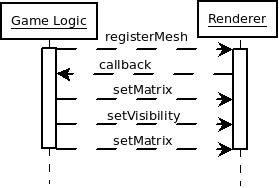
\includegraphics[scale=1]{zasoby/rozdzial31/renderer-messages}  
  \caption{Asynchroniczna komunikacja gry z rendererem}
  \label{fig:renderer-messages}
\end{figure}

Jak widać na schemacie \ref{fig:renderer-messages}, gra rejestruje na początku obiekt, który ma
być wyświetlony. Gdy rejestracja zostanie zakończona, renderer wysyła wiadomość zwrotną do gry.
Po zarejestrowaniu obiektu, renderer wyświetla go zgodnie z zapamiętanym stanem (macierz
transformacji, widoczność itd.), dopóki ten nie zostanie zmieniony.

Następnie komunikacja przepływa już tylko w jedną stronę. Gra wysyła komunikaty w celu zmiany
stanu obiektu w scenie 3d, bez oczekiwania na odpowiedź. Dzięki temu wątek gry wykonuje się
dalej podczas przekazywania i przetwarzania wiadomości. W celu dalszego zmniejszenia
narzutu wysyłania komend, są one kolejkowane po stronie gry i wysyłane większymi partiami
w jednej wiadomości.

Cały komunikacja jest opakowana w mechanizm zdalnego wywołania metod (rozdział \ref{ssec:zdalneWywolanie}),
dzięki czemu nie trzeba ręcznie tworzyć i wysyłać wiadomości. Dodatkowo, można łatwo przełączać
grę w tryb jednowątkowy w celu łatwiejszego wykrywania błędów i porównania wydajności.

\subsection{Struktura biblioteki renderera}

Diagram \ref{fig:renderer} prezentuje uproszczoną strukturę klas związanych z renderowaniem gry.

\begin{figure}[h!]
  \centering
  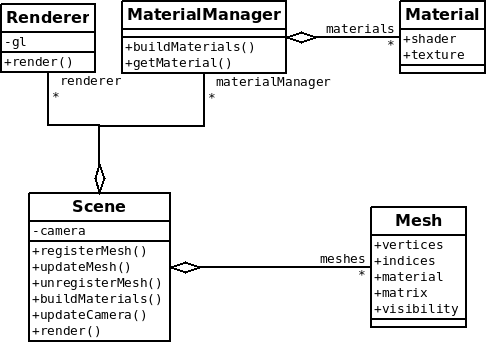
\includegraphics[scale=0.8]{zasoby/rozdzial31/renderer}  
  \caption{Uproszczony diagram klas związanych z rendererem}
  \label{fig:renderer}
\end{figure}

W następnych podrozdziałach znajduje się omówienie najważniejszych elementów biblioteki.

\subsubsection{Renderer}

Klasa o nazwie takiej samej jak nazwa całej biblioteki, odpowiada za bezpośrednią, niskopoziomową
komunikację z WebGL. Pośredniczy ona pomiędzy wysokopoziomową klasą sceny, operującej na
pojęciach obiektów, ich materiałów i pozycji, a niskopoziomowym API do rysowania trójkątów
za pomocą shaderów. Klasa renderera potrzebuje stanu obiektu, który otrzymuje od sceny
oraz materiał\footnote{Materiał graficzny -- zbiór właściwości opisujących wygląd obiektu, takich jak
kolor, tekstura, shader wykorzystywany do renderowania itp.}, przechowywany w menedżerze materiałów.

\subsubsection{Scena}

Klasą, która zarządza całym modułem renderera jest scena. Przechowuje ona stan wszystkich
zarejestrowanych przez grę obiektów graficznych oraz bezpośrednio odbiera i wykonuje
komendy zmiany stanu obiektu wysłane przez grę.

Po wywołaniu funkcji renderującej, scena przekazuje do niskopoziomowej klasy renderera
stan wszystkich obiektów razem z potrzebnymi

\subsubsection{Menedżer materiałów}

Do zadań menedżera materiałów należy tworzenie, przechowywanie i zarządzanie materiałami
graficznymi. Podczas inicjalizacji gry, menedżer tworzy potrzebne materiały. Podczas
ich tworzenia, konieczne jest między innymi wysłanie tekstur do pamięci karty graficznej
za pośrednictwem WebGL, a także skompilowanie używanych shaderów. Klasa ta dba również
o to, aby materiały nie dublowały się, zajmując niepotrzebnie pamięć.

\section{Zasoby gry}
\label{sec:zasobyGry}

WebArena wykorzystuje wiele rodzajów zasobów potrzebnych do wyświetlania grafiki i sterowania
logiką gry. Są to następujące pliki:
\begin{itemize}
\item pliki bsp z opisami poziomów gry,
\item pliki md3 z modelami 3d postaci, broni i innych przedmiotów,
\item opisy materiałów graficznych,
\item tekstury,
\item różnorakie pliki konfiguracyjne.
\end{itemize}

W związku z tym, że WebArena wykorzystuje zasoby gry OpenArena, wszystkie pliki są zgodne
z formatem używanym przez Quake III Arena. W dalszych podrozdziałach nastąpi omówienie
kodu odpowiedzialnego za wczytywanie zasobów wraz z pobieżnym omówieniem formatów plików.

\begin{figure}[h]
  \centering
  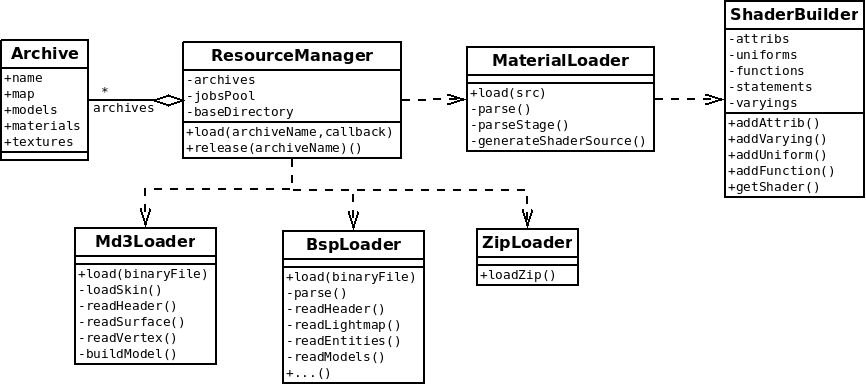
\includegraphics[scale=0.5]{zasoby/rozdzial31/resources}  
  \caption{Uproszczony diagram klas związanych z zarządzaniem zasobami.}
  \label{fig:screen}
\end{figure}

\subsection{Pliki BSP}

Pliki BSP służą do opisu geometrii i wyglądu poziomu. Format ten wywodzi się z Quake III. Nazwa
BSP oznacza Binary Space Partitioning i jest to również nazwa struktury danych (drzewo BSP),
w którym przechowywana jest geometria całego poziomu.
Drzewo BSP przyśpiesza wiele operacji wykonywanych w trakcie gry, a przede wszystkim wykrywanie
kolizji gracza lub pocisku z przedmiotami w świecie gry.

Kolejną ważną cechą plików BSP jest przechowywanie tzw. lightmapy, która służy do przedstawiania
realistycznego oświetlenia poziomu.

Plik BSP dzieli się na kilkanaście sekcji, przechowujących między innymi informacje o:
\begin{itemize}
\item budowie drzewa BSP,
\item wierzchołkach,
\item materiałach graficznych,
\item lightmapie,
\item efektach (takich jak np. mgła).
\end{itemize}

Dokładną specyfikację pliku BSP można znaleźć na na stronie \cite{bsp}. W WebArena do parsowania
pliku został częściowo wykorzystany kod z dema Brandona Jonesa opisanego w rozdziale \ref{ssec:quake3web}.

Ponieważ parsowanie pliku jest czasochłonne, jego wykonanie odbywa się na osobnym
wątku za pośrednictwem biblioteki opisanej w rozdziale \ref{sec:wielowatkowosc}.

\subsection{Pliki MD3}

MD3 jest formatem plików modeli graficznych używanym przez Quake III Arena. W plikach tych przechowywane
są wszystkie ruchome modele, takie jak postacie, bronie itp.

Ich ważną cechą jest możliwość przechowywania
animacji (w przeciwieństwie do plików BSP). Jest to animacja wierzchołkowa, w której dla każdej klatki
animacji, przechowywane są pozycje wszystkich wierzchołków. Sposób ten powoduje duże zużycie pamięci,
jednak jego zaletą jest prostota.

Kod do wczytywania plików MD3 został napisany specjalnie dla WebArena w oparciu o specyfikację dostępną 
na stronie \cite{md3} i tak jak w przypadku BSP, wykonywany jest na osobnym wątku.

\subsection{Pliki materiałów graficznych i tekstury}

Quake III Arena powstał w czasach gdy jeszcze niemożliwe było tworzenie shaderów. Na karcie graficznej
mógł działać tylko predefiniowany przez producenta program do renderowania, można było sterować jedynie
jego parametrami. Był to tzw. fixed pipeline.

Aby obejść ograniczenia tego rozwiązania i umożliwić grafikom elastyczne definiowanie wyglądu
powierzchni, id Tech 3 wprowadził pliki tekstowe z opisem materiałów graficznych, częściowo pełniących
również rolę dzisiejszych shaderów. Pliki te również były nazywane shaderami, co może wprowadzać
pewną niejasność, dlatego w tej pracy konsekwentnie będzie używane pojęcie materiału.

\begin{lstlisting}[caption=Przykładowy opis materiału]
models/powerups/ammo/machammo
{
	{
		map models/powerups/ammo/ammobox.tga
		rgbGen lightingDiffuse
	}
	{
		map models/powerups/ammo/ammolights.tga
		blendfunc blend
		rgbGen const ( 1 1 0 )
		alphaGen wave sawtooth 0 1 0 1 
	}
}
\end{lstlisting}

Dokładną specyfikację plików materiałów można znaleźć w \cite{q3shaders}.

Ponieważ przestarzały fixed pipeline jest całkowicie usunięty z OpenGL ES i WebGL, dlatego konieczne
było przetłumaczenie materiałów na kod shadera. Jest to realizowane podczas wczytywania materiału.
Większość kodu wczytującego i tłumaczącego materiały jest pobrane z pracy Brandona Jonesa (rozdział
\ref{ssec:quake3web}).

\subsection{Menedżer zasobów}

Menedżer zasobów zarządza wczytywaniem i przechowaniem zasobów z pomocą wyżej wymienionych parserów.
Wszystkie pliki wczytywane są asynchronicznie, za pomocą puli wątków opisanej w rozdziale \ref{ssec:puleWatkow}.
Dzięki temu interfejs użytkownika nie blokuje się nawet podczas wczytywania bardzo dużych plików.
Menedżer dba również, aby żaden plik nie został wczytany dwukrotnie, co oznaczałoby marnowanie
pamięci.

W przypadku gry sieciowej nie można pominąć kwestii przesyłania plików przez internet. Wszystkie
zasoby muszą być pobrane z serwera przed rozpoczęciem rozgrywki. Konieczne jest jednak maksymalne
skrócenie czasu oczekiwania gracza.

Ściąganie każdego pliku z osobna jest bardzo nieefektywne, z drugiej jednak strony pobieranie wszystkich
zasobów w jednym dużym archiwum trwało by zbyt długo. Dlatego trzeba podzielić pliki na kilka
archiwów, tak aby gracz pobierał jedynie te potrzebne do zagrania w dany poziom.

W tym celu został napisany skrypt działający po stronie serwera, który analizuje plik BSP lub MD3 i pakuje
go do jednego archiwum zip razem z wszystkimi plikami, do których się odwołuje (materiały, tekstury,
modele). Dzięki temu gra pobiera jedynie kilka plików zip, które są po stronie przeglądarki rozpakowywane.

Komunikacja odbywa się za pomocą technologii AJAX\footnote{AJAX (Asynchronous JavaScript and XML) -- technologia
służąca do wykonywania asynchronicznych zapytań HTML z języka JavaScript.}.

\section{Synchronizacja sieciowa}
\label{sec:synchronizacjaSieciowa}

\begin{figure}[h]
  \centering
  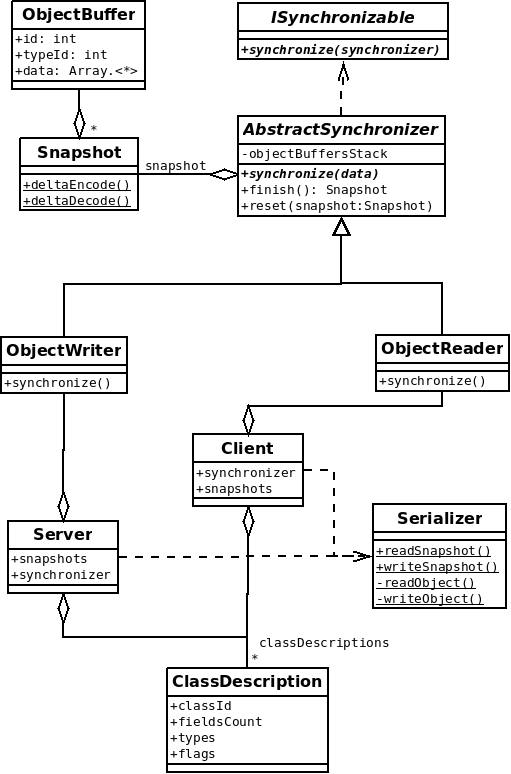
\includegraphics[scale=0.7]{zasoby/rozdzial31/network}  
  \caption{Diagram klas biblioteki do synchronizacji sieciowej.}
  \label{fig:screen}
\end{figure}


\section{Logika gry}
\label{sec:logikaGry}

\section{Opis z punktu widzenia użytkownika}

\begin{figure}[h]
  \centering
  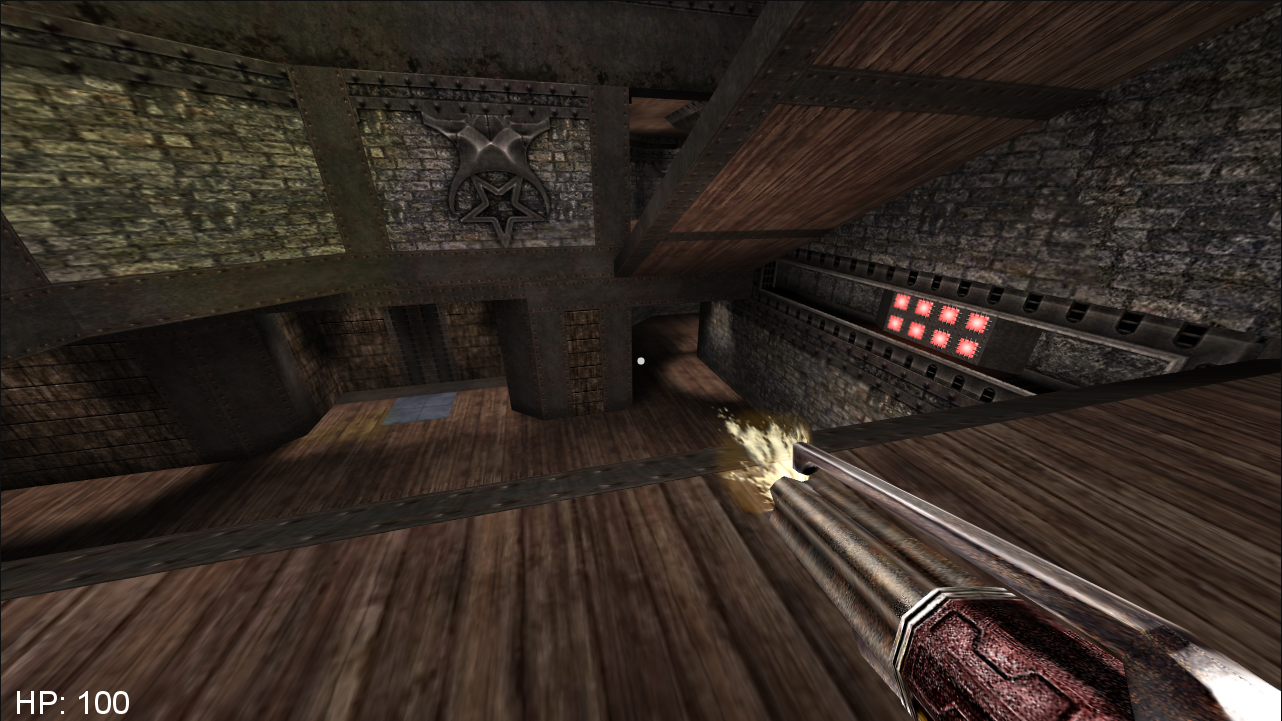
\includegraphics[scale=0.45]{zasoby/rozdzial31/screen}  
  \caption{Zrzut ekranu z gry Web Arena}
  \label{fig:screen}
\end{figure}


%%% Local Variables: 
%%% mode: latex
%%% TeX-master: "praca"
%%% End: 
